\chapter{Equalizer GPU Implementation}
\label{chap:equalizers_in_gpus}
Each equalizer in the PAQ system presents an interesting challenge from a GPU implementation perspective.
The equations for each equalizer in Section \ref{sec:equalizer_eq} were reformulated in preparation for fast and efficient GPU implementation.
This chapter is explain how the FIR equalizer filter coefficients are computed and applied.

Every equalizer filter is computed using batch processing.
In batch processing, each packet is totally independent of all other packets.
To simplify figures, every block diagram in this chapter shows how one packet is processed.
Each packet in a batch is processed exactly the same way with different data.
If a block diagram shows how to compute one equalizer filter, the block diagram is repeated $3104$ times compute a full batch of equalizer filters.

Convolution is used many times in this chapter.
Section \ref{sec:batched_convolution} showed that GPU frequency-domain batch convolution performs best for the PAQ system.
To simplify block diagrams, frequency -domain batch convolution is shown as one block.
Figures \ref{fig:Conv2} and \ref{fig:Conv3} show how frequency-domain batch convolution is represented in this chapter.

Note that the ``numerically optimized'' detection filter $\mathbf{h}_\text{NO}$ and the SOQPSK-TG power spectral density $\mathbf{\Psi}$ are defined constants.
The SOQPSK-TG power spectral density $\mathbf{\Psi}$ and $\mathbf{H}_\text{NO}$ are pre-computed and stored where $\mathbf{H}_\text{NO}$ is the $16$,$384$ point FFT of $\mathbf{h}_\text{NO}$.
Applying $\mathbf{h}_\text{NO}$ in the frequency domain does not require an extra FFT, only extra complex multiplies.
\begin{figure}
	\centering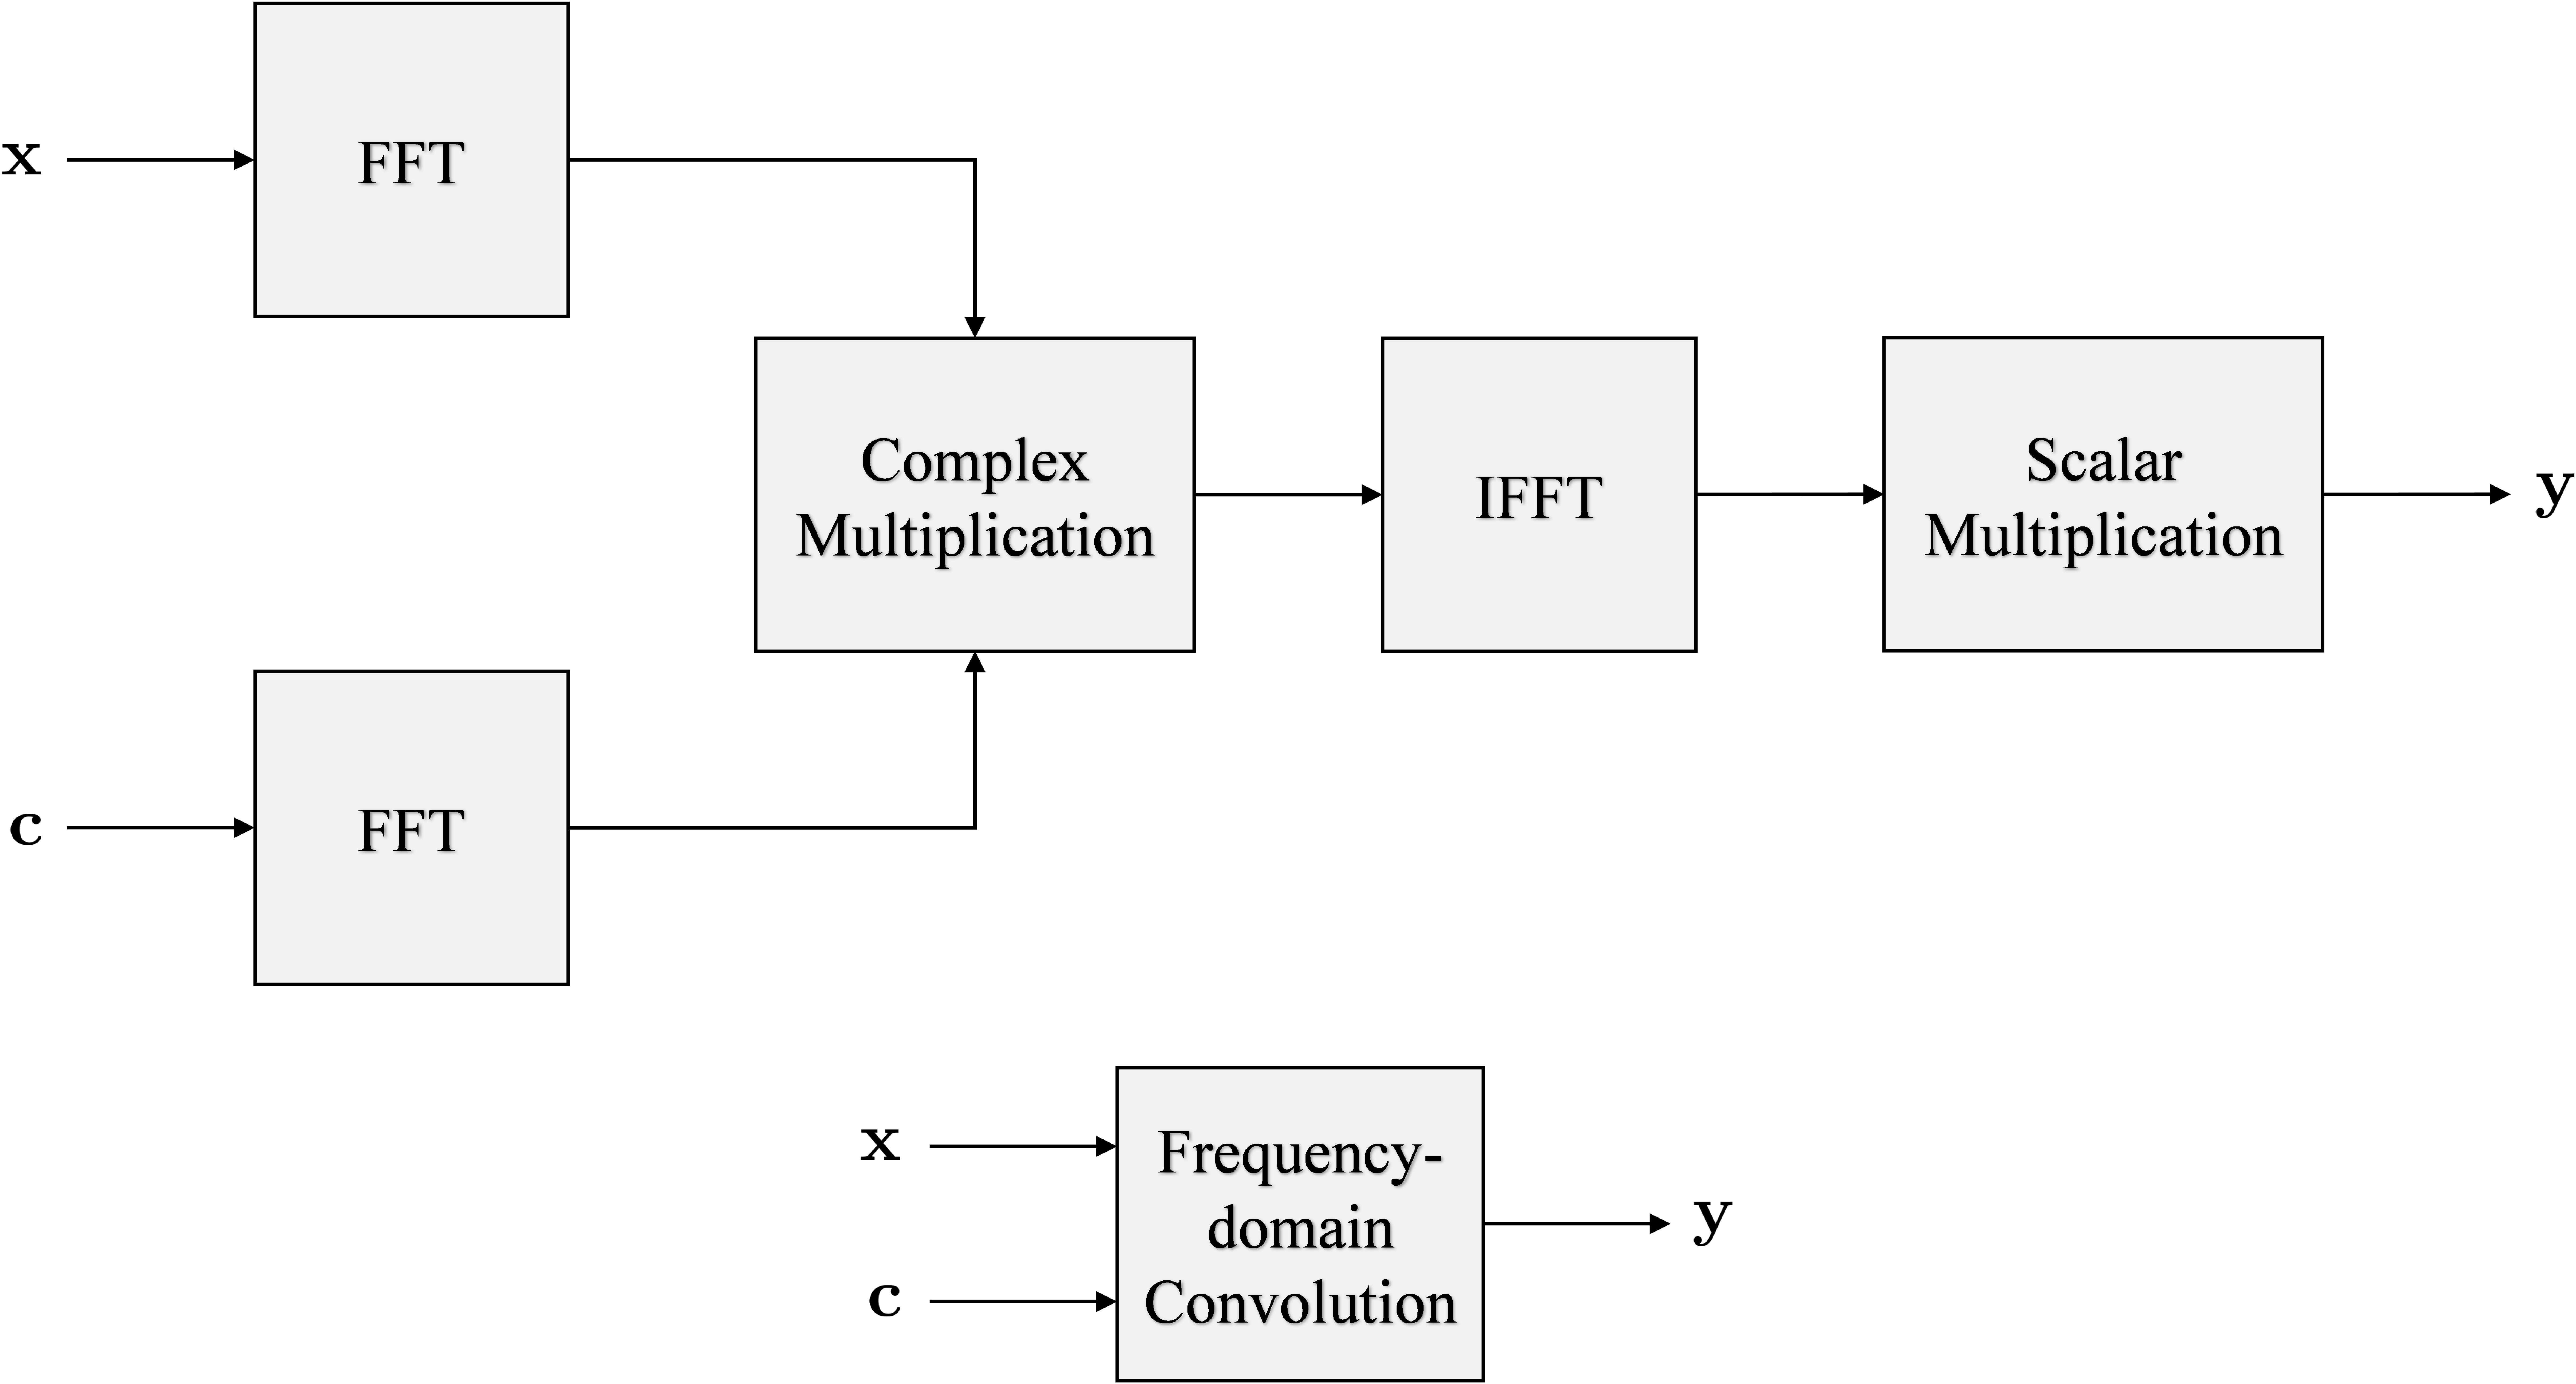
\includegraphics[width=10.28in/100*55]{figures/eq_GPUimplementation/Conv2.pdf}
	\caption{To simplify block diagrams, frequency-domain convolution is shown as one block.}
	\label{fig:Conv2}
\end{figure}
\begin{figure}
	\centering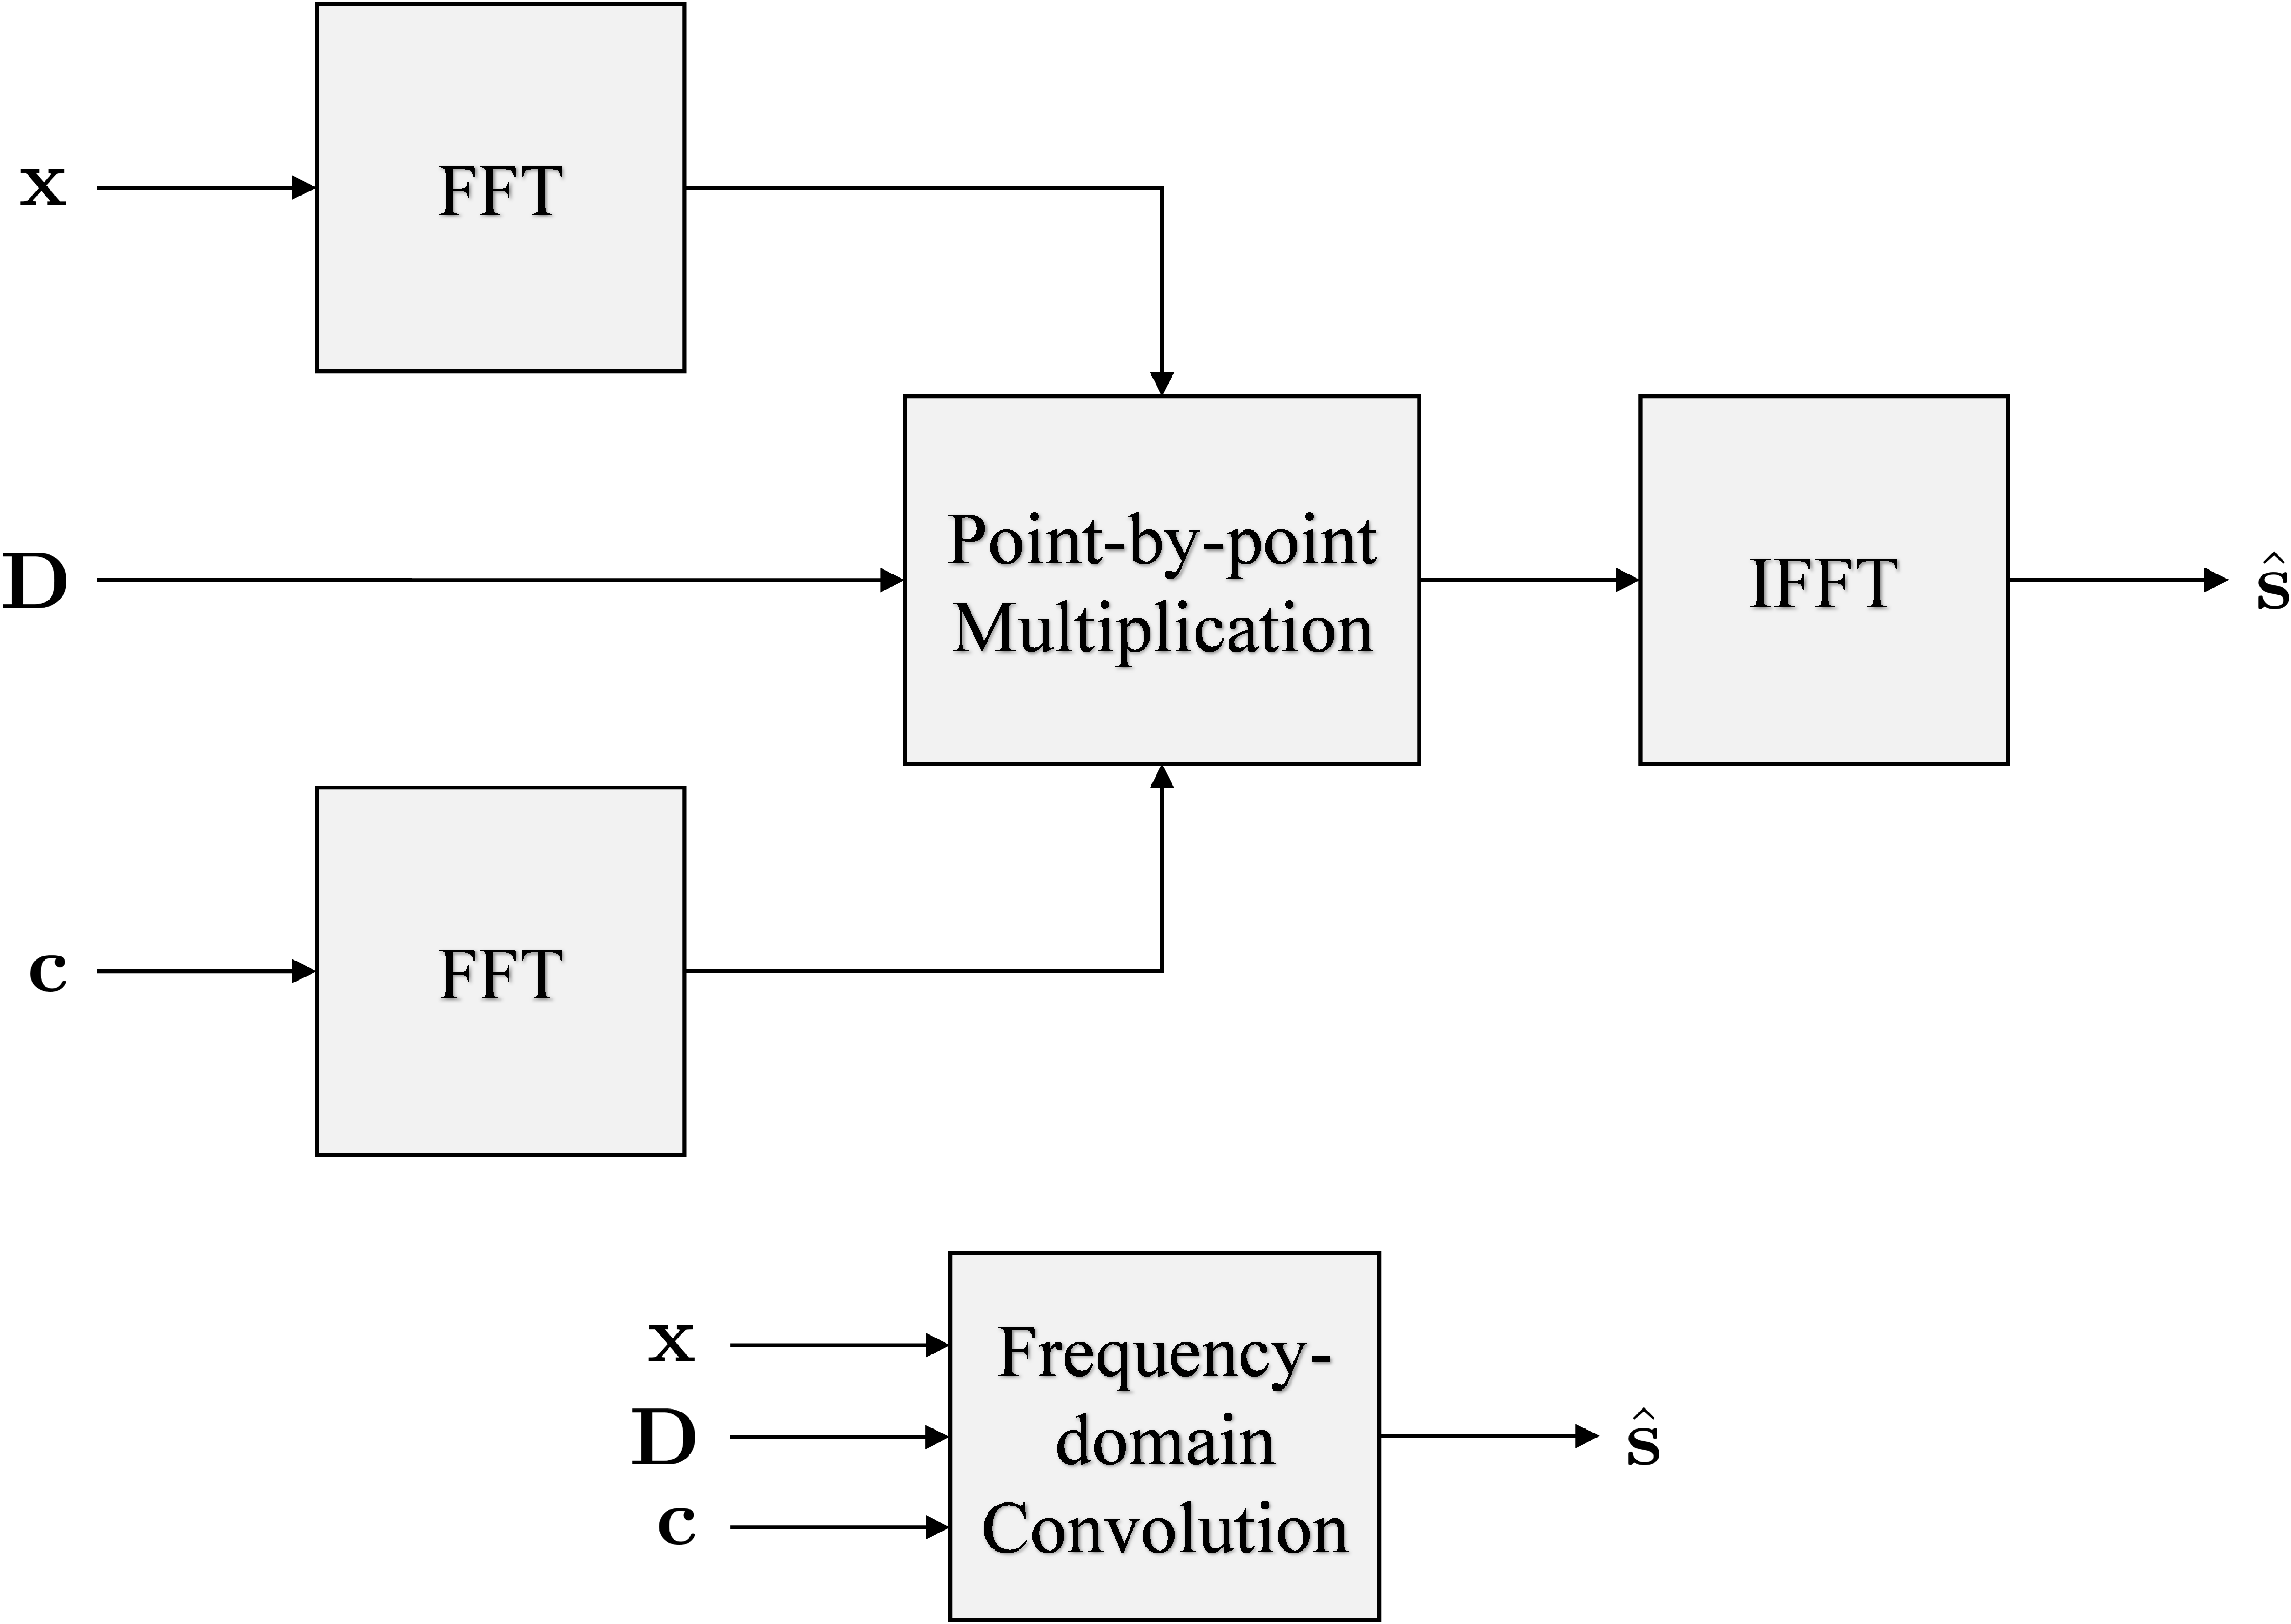
\includegraphics[width=10.28in/100*55]{figures/eq_GPUimplementation/Conv3.pdf}
	\caption{To simplify block diagrams, frequency-domain cascaded convolution is shown as one block.}
	\label{fig:Conv3}
\end{figure}

\clearpage
\section{Zero-Forcing and MMSE GPU Implementation}
%The ZF equalizer is an FIR filter defined by the coefficients
%\begin{equation}
%\begin{matrix}
%c_\text{ZF}(-L_1) & \cdots & c_\text{ZF}(0) & \cdots & c_\text{ZF}(L_2).
%\end{matrix}
%\end{equation}
%The filter coefficients are the solution to the matrix vector equation \cite[eq. (311)]{PAQ-phase1}
%\begin{equation}
%\mathbf{c}_\text{ZF} = \big(\mathbf{H}^\dagger\mathbf{H}\big)^{-1} \mathbf{H}^\dagger \mathbf{u}_{n_0}
%\label{eq:c_ZF_direct}
%\end{equation}
%where
%\begin{equation}
%\mathbf{c}_\text{ZF} = 
%\begin{bmatrix}
%c_\text{ZF}(-L_1) \\ \vdots \\ c_\text{ZF}(0) \\ \vdots \\ c_\text{ZF}(L_2)
%\end{bmatrix},
%\end{equation}
%\begin{equation}
%\mathbf{u}_{n_0} = \begin{bmatrix} 0 \\ \vdots \\ 0 \\ 1 \\ 0 \\ \vdots \\ 0 \end{bmatrix}
%	\begin{matrix*}[l] \left. \vphantom{\begin{matrix} 0 \\ \vdots \\ 0 \end{matrix}} \right\}
%		\text{$n_0-1$ zeros}
%		\\ \\
%		\left. \vphantom{\begin{matrix} 0 \\ \vdots \\ 0 \end{matrix}} \right\}
%		\text{$N_1+N_2+L_1+L_2-n_0+1$ zeros}
%		\end{matrix*},
%		\label{eq:un0_ZF}
%\end{equation}
%where $n_0 = N_1+L_1+1$ and
%\begin{equation} 
%\mathbf{H} = 
%		\begin{bmatrix}
%		\hat{h}(-N_1)		&  				& 		 	&  					\\
%		\hat{h}(-N_1+1) 	& \hat{h}(-N_1)	& 		 	&  					\\
%		\vdots	 			& \vdots		& \ddots 	&  					\\
%		\hat{h}(N_2)		& \hat{h}(N_2-1)&  			& \hat{h}(-N_1)  	\\
%		 					& \hat{h}(N_2) 	&  			& \hat{h}(-N_1+1) 	\\
%		 					&  	   			&  			& \vdots			\\
%		 					&  	   			&  			& \hat{h}(N_2)		\\
%	\end{bmatrix}.
%\end{equation}
%
%Equation \eqref{eq:c_ZF_direct} can be implemented directly but there are many optimization that greatly reduce computation.
%The heaviest computation is the $\mathcal{O}(n^3)$ inverse operation followed by the $\mathcal{O}(n^2)$ matrix matrix multiplies.
%Rather than performing a heavy inverse, multiplying $\mathbf{H}^\dagger \mathbf{H}$ on both sides of equation \eqref{eq:c_ZF_direct} results in
%\begin{align}
%\mathbf{H}^\dagger\mathbf{H} \mathbf{c}_\text{ZF} &= \mathbf{H}^\dagger \mathbf{u}_{n_0} \nonumber \\
%\mathbf{R}_{\hat{h}} \mathbf{c}_\text{ZF} &= \hat{\mathbf{h}}_{n_0}
%\label{eq:c_ZF_solve}
%\end{align}
%where
%\begin{equation}
%\mathbf{R}_{\hat{h}} = 
%\mathbf{H}^\dagger \mathbf{H} = 
%		\begin{bmatrix}
%		r_{\hat{h}}(0)			& r^\ast_{\hat{h}}(1)	& \cdots 	& r^\ast_{\hat{h}}(L_{eq}-1)  	\\
%		r_{\hat{h}}(1) 			& r_{\hat{h}}(0)		& \cdots 	& r^\ast_{\hat{h}}(L_{eq}-2)  	\\
%		\vdots	 				& \vdots				& \ddots 	&  								\\
%		r_{\hat{h}}(L_{eq}-1)	& r_{\hat{h}}(L_{eq}-2)	& \cdots	& r_{\hat{h}}(0)  			
%	\end{bmatrix}
%	\label{eq:R_h}
%\end{equation}
%is the auto-correlation matrix of the channel estimate $\hat{\mathbf{h}}$
%and 
%\begin{equation}
%\hat{\mathbf{h}}_{n_0} = \mathbf{H}^\dagger \mathbf{u}_{n_0} = 
%\begin{bmatrix} \hat{h}^\ast(L_1) \\ \vdots \\ \hat{h}^\ast(0) \\ \vdots \\ \hat{h}^\ast(-L_2)  \end{bmatrix}
%\label{eq:h_no}
%\end{equation}
%is a vector with the time reversed and conjugated channel estimate $\hat{\mathbf{h}}$ centered at $n_0$.
%The channel estimate auto-correlation sequence is
%\begin{equation}
%r_{\hat{h}}(k) = \sum_{n=-N_1}^{N_2} \hat{h}(n) \hat{h}^\ast(n-k).
%\label{eq:sample_autocorrelation}
%\end{equation}
%Note that the auto-correlation matrix $\mathbf{R}_{\hat{h}}$ is comprised of 
%\begin{equation}
%\mathbf{r}_{\hat{h}} = 
%\begin{bmatrix} r_{\hat{h}}(0) \\ \vdots \\ r_{\hat{h}}(L_{ch}) \\ r_{\hat{h}}(L_{ch}+1) \\ \vdots \\ r_{\hat{h}}(L_{eq}-1)\end{bmatrix} =
%\begin{bmatrix} r_{\hat{h}}(0) \\ \vdots \\ r_{\hat{h}}(L_{ch}) \\ 0 \\ \vdots \\ 0  \end{bmatrix}.
%\end{equation} 
%Using $\mathbf{r}_{\hat{h}}$ eliminates the need for matrix matrix multiply of $\mathbf{H}^\dagger\mathbf{H}$.
%Also, $r_{\hat{h}}(k)$ only has support on $-(L_{ch}-1) \leq k \leq L_{ch}-1$ making $\mathbf{R}_{\hat{h}}$ sparse or $\%63$ zeros. NEEDS CHECKING!!!!
%The sparseness of $\mathbf{R}_{\hat{h}}$ can be leveraged to reduce computation drastically.
%
%The MMSE equalizer is an FIR filter defined by the coefficients
%\begin{equation}
%\begin{matrix}
%c_\text{MMSE}(-L_1) & \cdots & c_\text{MMSE}(0) & \cdots & c_\text{MMSE}(L_2).
%\end{matrix}
%\end{equation}
%The filter coefficients are the solution to the matrix vector equation \cite[eq. (330) and (333)]{PAQ-phase1}
%\begin{equation}
%\mathbf{c}_\text{MMSE} = \big[ \mathbf{G}\mathbf{G}^\dagger + 2\hat{\sigma}^2_w\mathbf{I}_{L_1+L_2+1} \big]^{-1} \mathbf{g}^\dagger
%\label{eq:c_MMSE_direct}
%\end{equation}
%where $\mathbf{I}_{L_1+L_2+1}$ is the $(L_1+L_2+1)\times(L_1+L_2+1)$ identity matrix,
%$\hat{\sigma}^2_w$ is the estimated noise variance, $\mathbf{G}$ is the $(L_1+L_2+1)\times(N_1+N_2+L_1+L_2+1)$ matrix given by
%\begin{equation}
%\mathbf{G} = 
%		\begin{bmatrix}
%		\hat{h}(N_2)		& \cdots		& \hat{h}(-N_1) 	&  				  \\
%							& \hat{h}(N_2)	& \cdots 			& \hat{h}(-N_1)	  \\
%				 			& 				& \ddots 			&  				& \ddots	  \\
%		 					&  	   			&  					& \hat{h}(N_2)	& \cdots	& \hat{h}(-N_1)	\\
%	\end{bmatrix}
%\end{equation}
%and $\mathbf{g}^\dagger$ is the $(L_1+L_2+1)\times1$ vector given by
%\begin{equation}
%\mathbf{g}^\dagger = \hat{\mathbf{h}}_{n0} = \begin{bmatrix} \hat{h}^\ast(L_1) \\ \vdots \\ \hat{h}^\ast(0) \\ \vdots \\ \hat{h}^\ast(-L_2)  \end{bmatrix}.
%%\begin{bmatrix} \hat{h}(L_1) \cdots \hat{h}(-L_2) \end{bmatrix}.
%\label{eq:g_dagger_h_n0}
%\end{equation}
%
%Computing $\mathbf{c}_\text{MMSE}$ can be simplified by noticing that $\mathbf{g}^\dagger = \hat{\mathbf{h}}_{n_0}$, $\mathbf{G}\mathbf{G}^\dagger = \mathbf{R}_{\hat{h}}$ in Equation \eqref{eq:R_h}.
%To further simplify MMSE, twice the estimated noise variance is added down the diagonal of the channel estimate auto-correlation matrix
%\begin{equation}
%\mathbf{R} = 
%\mathbf{R}_{\hat{h}} + 2\hat{\sigma^2_w} \mathbf{I}_{L_1+L_2+1} = 
%		\begin{bmatrix}
%		r_{h}(0) + 2\hat{\sigma^2_w}	& r^\ast_{h}(1)							& \cdots 	& r^\ast_{h}(L_{eq}-1)  	\\
%		r_{h}(1) 						& r_{h}(0) + 2\hat{\sigma^2_w}& \cdots 	& r^\ast_{h}(L_{eq}-2)  				\\
%		\vdots	 						& \vdots								& \ddots 	&  							\\
%		r_{h}(L_{eq}-1)					& r_{h}(L_{eq}-2)						& \cdots	& r_{h}(0) + 2\hat{\sigma^2_w}  			
%	\end{bmatrix}.
%	\label{eq:R_MMSE}
%\end{equation}
%By placing Equation \eqref{eq:R_MMSE} and \eqref{eq:g_dagger_h_n0} into \eqref{eq:c_MMSE_direct} results in
%\begin{equation}
%\mathbf{c}_\text{MMSE} = \mathbf{R}^{-1} \hat{\mathbf{h}}_{n_0}.
%\end{equation}
%Solving for the MMSE equalizer coefficients $\mathbf{c}_\text{MMSE}$ takes the form like the ZF equalizer coeffiencts in \eqref{eq:c_ZF_solve}
%\begin{equation}
%\mathbf{R}\mathbf{c}_\text{MMSE} = \hat{\mathbf{h}}_{n_0}.
%\label{eq:c_MMSE_solve}
%\end{equation}
%
%The only difference between solving for the ZF and MMSE equalizer coefficients is $\mathbf{R}$ and $\mathbf{R}_{\hat{h}}$. 
%The MMSE equalizer coefficients $\mathbf{c}_\text{MMSE}$ uses the noise variance estimate when building $\mathbf{R}$.
%The sparseness of $\mathbf{R}$ can also be leveraged to reduce computation drastically because
%$\mathbf{R}$ has the same sparse properties as $\mathbf{R}_{\hat{h}}$.

The ZF and MMSE FIR equalizer filter coefficient computations have exactly the same form as shown in Equations \eqref{eq:start_here_ZF} and \eqref{eq:start_here_MMSE}.
Any ZF equalizer filter computation restructuring can also be applied directly to the MMSE equalizer filter computation.
To simplify the conversation, the following section will explain the investigation only the ZF equalizer filter GPU implementation.

The ZF equalizer filter can be computed two ways: solve the system of linear equations 
\begin{equation}
\mathbf{R}_{\hat{h}} \mathbf{c}_\text{ZF} = \hat{\mathbf{h}}_{n_0}
\label{eq:start_here_ZF_gpuimp}
\end{equation}
or compute the inverse of $\mathbf{R}_{\hat{h}}$ then perform matrix vector multiplication
\begin{equation}
\mathbf{c}_\text{ZF} =\mathbf{R}^{-1}_{\hat{h}} \hat{\mathbf{h}}_{n_0}.
\label{eq:c_ZF_direct}
\end{equation}
Both techniques require $\mathcal{O}(n^3)$ operations making the computation of the ZF and MMSE equalizer filter coefficients extremely heavy.
Computing a matrix inverse or solving linear systems in GPUs is especially challenging because common algorithms for matrix inversion and solving linear systems are serial.
Three approaches to computing the equalizer filter coefficients were explored
\begin{itemize}
\item Using the Levinson-Durbin recursion algorithm to solve the system of equations
\item Using the cuBLAS LU decomposition library to compute the inverse and matrix vector multiplication
\item Using the cuSolver library to solve the system of equations.
\end{itemize}

The Levinson-Durbin recursion algorithm avoids $\mathcal{O}(n^3)$ inverse or solving operations by leveraging the Toeplitz or diagonal-constant structure of $\mathbf{R}_{\hat{h}}$ \cite[Chap. 5]{hayes:1996}.
The first GPU implementation of the Levinson-Durbin recursion algorithm computed the ZF equalizer filter assuming the matrix $\mathbf{R}_{\hat{h}}$ and the vector $\hat{\mathbf{h}}_{n_0}$ were \textit{real-valued}.
The Levinson-Durbin recursion algorithm showed promise by computing $3104$ real-valued ZF equalizer filters in $500$ ms.

The GPU implementation of Levinson-Durbin recursion was then converted from computing real-valued ZF equalizer filters to computing \textit{complex-valued} ZF equalizer filters.
Converting from real-valued to complex-valued filters requires more memory accesses and flops.
The Levinson-Durbin recursion computed $3104$ complex-valued ZF equalizer filters in $2$,$500$ ms, in excess of the $1907$ ms maximum for all processing time.

The next algorithm explored computed the inverse of $\mathbf{R}_{\hat{h}}$ using the cuBLAS batch processing library.
The cuBLAS library computes a \textit{complex-valued} inverse using the LU decomposition in $600$ ms.
cuBLAS executed faster than the Levinson-Durbin recursion algorithm but $600$ ms is still $31\%$ of the total $1907$ ms processing time.

The final and fastest algorithm explored solves the linear system in Equation \eqref{eq:start_here_ZF_gpuimp}using a GPU sparse complex-valued solver library called cuSolverSp.
A sparse solver can be used because section \ref{sec:ZFnMMSE} showed that $\mathbf{R}_{\hat{h}}$ is sparse comprising $63\%$ zeros because the matrix comprises of the vector $\mathbf{r}_{\hat{h}}$ with finite support on $-(L_{ch}-1) \leq k \leq L_{ch}-1$.

``cusolverSpCcsrqrsvBatched'' is the GPU function used from the cuSolverSp library.
cusolverSpCcsrqrsvBatched is a complex-valued batch solver that leverages the sparse properties of $\mathbf{R}_{\hat{h}}$ by exploiting Compressed Row Storage (CRS) \cite{wiki:Sparse_matrix}.
Compressed Row Storage reduces the large $186\times186$ matrices to a $12544$ element CSR matrix $\mathbf{R}_{\hat{h}\text{CRS}}$.
Before cusolverSpCcsrqrsvBatched can be called, the CSR matrix $\mathbf{R}_{\hat{h}\text{CRS}}$ has to be built using $\mathbf{r}_{\hat{h}}$.
An example of how to use the CUDA cusolverSp library can be found in \cite{CUDA_toolkit_doc}.
Before the cuSolverSp library can be called, the CSR matrix $\mathbf{R}_{\hat{h}\text{CRS}}$ must be built from the estimated channel auto-correlation and the vector $\hat{\mathbf{h}}_{n_0}$ is built with the conjugated and time-reversed estimated channel $\mathbf{\hat{h}}$. 

Figures \ref{fig:blockZF} and \ref{fig:blockMMSE} show how the ZF and MMSE equalizer filters are computed and applied to the received samples.
Note that the equalizer filters are applied in the frequency-domain with the detection filter.
\begin{figure}
	\centering\includegraphics[width=7.5in/100*55]{figures/eq_GPUimplementation/blockZF.pdf}
	\caption{Block Diagram showing how the Zero-Forcing equalizer coefficients are implemented in the GPU.}
	\label{fig:blockZF}
\end{figure}
\begin{figure}
	\centering\includegraphics[width=7.98in/100*55]{figures/eq_GPUimplementation/blockMMSE.pdf}
	\caption{Block Diagram showing how the Minimum Mean Squared Error equalizer coefficients are implemented in the GPU.}
	\label{fig:blockMMSE}
\end{figure}
Table \ref{tab:ZFMMSEtimingComparison} lists the algorithms researched and their respective execution times.
\begin{table}
\caption{Three different algorithms were explored to compute the ZF and MMSE equalizer filters.}
\begin{center}
\begin{tabular}{lll}
	\toprule
	Algorithm 			& Data type	& Execution Time (ms)	\\ \midrule
	Levinson Recursion 	& floats 	& 500 					\\
	Levinson Recursion 	& Complex 	& 2500 					\\
	LU Decomposition 	& Complex 	& 600				 	\\
	cuSolver			& Complex	& 355.96				\\
	\bottomrule
\end{tabular}
\end{center}
\label{tab:ZFMMSEtimingComparison}
\end{table}

%
%
%
%The ZF equalizer filter can be computed two ways: solve the system of linear equations shown in Equation \eqref{eq:c_ZF_direct} or compute the inverse of $\mathbf{R}_{\hat{h}}$ then perform matrix vector multiplication
%\begin{equation}
%\mathbf{c}_\text{ZF} =\mathbf{R}^{-1}_{\hat{h}} \hat{\mathbf{h}}_{n_0}
%\label{eq:c_ZF_direct}
%\end{equation}
%where 
%\begin{equation}
%\mathbf{R}_{\hat{h}} = 
%		\begin{bmatrix}
%		r_{\hat{h}}(0)			& r^\ast_{\hat{h}}(1)	& \cdots 	& r^\ast_{\hat{h}}(L_{eq}-1)  	\\
%		r_{\hat{h}}(1) 			& r_{\hat{h}}(0)		& \cdots 	& r^\ast_{\hat{h}}(L_{eq}-2)  	\\
%		\vdots	 				& \vdots				& \ddots 	&  								\\
%		r_{\hat{h}}(L_{eq}-1)	& r_{\hat{h}}(L_{eq}-2)	& \cdots	& r_{\hat{h}}(0)  			
%	\end{bmatrix}.
%	\label{eq:R_h}
%\end{equation}
%The matrix $\mathbf{R}_{\hat{h}}$ is the auto-correlation matrix of the channel estimate $\hat{\mathbf{h}}$
%and 
%\begin{equation}
%\hat{\mathbf{h}}_{n_0} = \mathbf{H}^\dagger \mathbf{u}_{n_0} = 
%\begin{bmatrix} \hat{h}^\ast(L_1) \\ \vdots \\ \hat{h}^\ast(0) \\ \vdots \\ \hat{h}^\ast(-L_2)  \end{bmatrix}
%\label{eq:h_no}
%\end{equation}
%is a vector with the time reversed and conjugated channel estimate $\hat{\mathbf{h}}$ centered at $n_0$.
%The channel estimate auto-correlation sequence is
%\begin{equation}
%r_{\hat{h}}(k) = \sum_{n=-N_1}^{N_2} \hat{h}(n) \hat{h}^\ast(n-k).
%\label{eq:sample_autocorrelation}
%\end{equation}
%Note that the auto-correlation matrix $\mathbf{R}_{\hat{h}}$ is comprised of 
%\begin{equation}
%\mathbf{r}_{\hat{h}} = 
%\begin{bmatrix} r_{\hat{h}}(0) \\ \vdots \\ r_{\hat{h}}(L_{ch}) \\ r_{\hat{h}}(L_{ch}+1) \\ \vdots \\ r_{\hat{h}}(L_{eq}-1)\end{bmatrix} =
%\begin{bmatrix} r_{\hat{h}}(0) \\ \vdots \\ r_{\hat{h}}(L_{ch}) \\ 0 \\ \vdots \\ 0  \end{bmatrix}.
%\end{equation} 
%Using $\mathbf{r}_{\hat{h}}$ eliminates the need for matrix matrix multiply of $\mathbf{H}^\dagger\mathbf{H}$.
%Also, $r_{\hat{h}}(k)$ only has support on $-(L_{ch}-1) \leq k \leq L_{ch}-1$ making $\mathbf{R}_{\hat{h}}$ sparse or $\%63$ zeros. NEEDS CHECKING!!!!
%The sparseness of $\mathbf{R}_{\hat{h}}$ can be leveraged to reduce computation drastically.
%
%
%\clearpage
%
%lizer is an FIR filter defined by the coefficients
%\begin{equation}
%\begin{matrix}
%c_\text{ZF}(-L_1) & \cdots & c_\text{ZF}(0) & \cdots & c_\text{ZF}(L_2).
%\end{matrix}
%\end{equation}
%The filter coefficients are the solution to the matrix vector equation \cite[eq. (311)]{PAQ-phase1}
%\begin{equation}
%\mathbf{c}_\text{ZF} = \big(\mathbf{H}^\dagger\mathbf{H}\big)^{-1} \mathbf{H}^\dagger \mathbf{u}_{n_0}
%\label{eq:c_ZF_direct}
%\end{equation}
%where
%\begin{equation}
%\mathbf{c}_\text{ZF} = 
%\begin{bmatrix}
%c_\text{ZF}(-L_1) \\ \vdots \\ c_\text{ZF}(0) \\ \vdots \\ c_\text{ZF}(L_2)
%\end{bmatrix},
%\end{equation}
%\begin{equation}
%\mathbf{u}_{n_0} = \begin{bmatrix} 0 \\ \vdots \\ 0 \\ 1 \\ 0 \\ \vdots \\ 0 \end{bmatrix}
%	\begin{matrix*}[l] \left. \vphantom{\begin{matrix} 0 \\ \vdots \\ 0 \end{matrix}} \right\}
%		\text{$n_0-1$ zeros}
%		\\ \\
%		\left. \vphantom{\begin{matrix} 0 \\ \vdots \\ 0 \end{matrix}} \right\}
%		\text{$N_1+N_2+L_1+L_2-n_0+1$ zeros}
%		\end{matrix*},
%		\label{eq:un0_ZF}
%\end{equation}
%where $n_0 = N_1+L_1+1$ and
%\begin{equation} 
%\mathbf{H} = 
%		\begin{bmatrix}
%		\hat{h}(-N_1)		&  				& 		 	&  					\\
%		\hat{h}(-N_1+1) 	& \hat{h}(-N_1)	& 		 	&  					\\
%		\vdots	 			& \vdots		& \ddots 	&  					\\
%		\hat{h}(N_2)		& \hat{h}(N_2-1)&  			& \hat{h}(-N_1)  	\\
%		 					& \hat{h}(N_2) 	&  			& \hat{h}(-N_1+1) 	\\
%		 					&  	   			&  			& \vdots			\\
%		 					&  	   			&  			& \hat{h}(N_2)		\\
%	\end{bmatrix}.
%\end{equation}
%
%Equation \eqref{eq:c_ZF_direct} can be implemented directly but there are many optimization that greatly reduce computation.
%The heaviest computation is the $\mathcal{O}(n^3)$ inverse operation followed by the $\mathcal{O}(n^2)$ matrix matrix multiplies.
%Rather than performing a heavy inverse, multiplying $\mathbf{H}^\dagger \mathbf{H}$ on both sides of equation \eqref{eq:c_ZF_direct} results in
%\begin{align}
%\mathbf{H}^\dagger\mathbf{H} \mathbf{c}_\text{ZF} &= \mathbf{H}^\dagger \mathbf{u}_{n_0} \nonumber \\
%\mathbf{R}_{\hat{h}} \mathbf{c}_\text{ZF} &= \hat{\mathbf{h}}_{n_0}
%\label{eq:c_ZF_solve}
%\end{align}
%where
%\begin{equation}
%\mathbf{R}_{\hat{h}} = 
%\mathbf{H}^\dagger \mathbf{H} = 
%		\begin{bmatrix}
%		r_{\hat{h}}(0)			& r^\ast_{\hat{h}}(1)	& \cdots 	& r^\ast_{\hat{h}}(L_{eq}-1)  	\\
%		r_{\hat{h}}(1) 			& r_{\hat{h}}(0)		& \cdots 	& r^\ast_{\hat{h}}(L_{eq}-2)  	\\
%		\vdots	 				& \vdots				& \ddots 	&  								\\
%		r_{\hat{h}}(L_{eq}-1)	& r_{\hat{h}}(L_{eq}-2)	& \cdots	& r_{\hat{h}}(0)  			
%	\end{bmatrix}
%	\label{eq:R_h}
%\end{equation}
%is the auto-correlation matrix of the channel estimate $\hat{\mathbf{h}}$
%and 
%\begin{equation}
%\hat{\mathbf{h}}_{n_0} = \mathbf{H}^\dagger \mathbf{u}_{n_0} = 
%\begin{bmatrix} \hat{h}^\ast(L_1) \\ \vdots \\ \hat{h}^\ast(0) \\ \vdots \\ \hat{h}^\ast(-L_2)  \end{bmatrix}
%\label{eq:h_no}
%\end{equation}
%is a vector with the time reversed and conjugated channel estimate $\hat{\mathbf{h}}$ centered at $n_0$.
%The channel estimate auto-correlation sequence is
%\begin{equation}
%r_{\hat{h}}(k) = \sum_{n=-N_1}^{N_2} \hat{h}(n) \hat{h}^\ast(n-k).
%\label{eq:sample_autocorrelation}
%\end{equation}
%Note that the auto-correlation matrix $\mathbf{R}_{\hat{h}}$ is comprised of 
%\begin{equation}
%\mathbf{r}_{\hat{h}} = 
%\begin{bmatrix} r_{\hat{h}}(0) \\ \vdots \\ r_{\hat{h}}(L_{ch}) \\ r_{\hat{h}}(L_{ch}+1) \\ \vdots \\ r_{\hat{h}}(L_{eq}-1)\end{bmatrix} =
%\begin{bmatrix} r_{\hat{h}}(0) \\ \vdots \\ r_{\hat{h}}(L_{ch}) \\ 0 \\ \vdots \\ 0  \end{bmatrix}.
%\end{equation} 
%Using $\mathbf{r}_{\hat{h}}$ eliminates the need for matrix matrix multiply of $\mathbf{H}^\dagger\mathbf{H}$.
%Also, $r_{\hat{h}}(k)$ only has support on $-(L_{ch}-1) \leq k \leq L_{ch}-1$ making $\mathbf{R}_{\hat{h}}$ sparse or $\%63$ zeros. NEEDS CHECKING!!!!
%The sparseness of $\mathbf{R}_{\hat{h}}$ can be leveraged to reduce computation drastically.
%
%
%\clearpage
%Equations \eqref{eq:start_here_ZF_gpuimp} and \eqref{eq:start_here_MMSE_gpuimp} can be solved 
%
%The equalizer filter coefficients $\mathbf{c}_\text{ZF}$ and $\mathbf{c}_\text{MMSE}$ can be computed in two ways: solve the linear system of equations in Equations \eqref{eq:start_here_ZF_gpuimp} and \eqref{eq:start_here_MMSE_gpuimp} or 
%\begin{equation}
%\mathbf{c}_\text{ZF} =\mathbf{R}^{-1}_{\hat{h}} \hat{\mathbf{h}}_{n_0}
%\label{eq:c_ZF_direct}
%\end{equation}
%\begin{equation}
%\mathbf{c}_\text{MMSE} = \mathbf{R}^{-1} \hat{\mathbf{h}}_{n_0}
%\label{eq:c_MMSE_direct}
%\end{equation}
%compute the inverse of $\mathbf{R}_{\hat{h}}$ and $\mathbf{R}$ then perform matrix vector multiplication with the vector $\hat{\mathbf{h}}_{n_0}$.
%
%Equation \eqref{eq:c_ZF_direct} and \eqref{eq:c_MMSE_direct} can be implemented directly but there are many ways to greatly reduce computation.
%
%
%The heaviest computation is the $\mathcal{O}(n^3)$ inverse operation followed by the $\mathcal{O}(n^2)$ matrix matrix multiplies.
%
%Equation \eqref{eq:c_ZF_direct} can be implemented directly but there are many optimization that greatly reduce computation.
%The heaviest computation is the $\mathcal{O}(n^3)$ inverse operation followed by the $\mathcal{O}(n^2)$ matrix matrix multiplies.
%Rather than performing a heavy inverse, multiplying $\mathbf{H}^\dagger \mathbf{H}$ on both sides of equation \eqref{eq:c_ZF_direct} results in
%\begin{align}
%\mathbf{H}^\dagger\mathbf{H} \mathbf{c}_\text{ZF} &= \mathbf{H}^\dagger \mathbf{u}_{n_0} \nonumber \\
%\mathbf{R}_{\hat{h}} \mathbf{c}_\text{ZF} &= \hat{\mathbf{h}}_{n_0}
%\label{eq:c_ZF_solve}
%\end{align}
%where
%\begin{equation}
%\mathbf{R}_{\hat{h}} = 
%\mathbf{H}^\dagger \mathbf{H} = 
%		\begin{bmatrix}
%		r_{\hat{h}}(0)			& r^\ast_{\hat{h}}(1)	& \cdots 	& r^\ast_{\hat{h}}(L_{eq}-1)  	\\
%		r_{\hat{h}}(1) 			& r_{\hat{h}}(0)		& \cdots 	& r^\ast_{\hat{h}}(L_{eq}-2)  	\\
%		\vdots	 				& \vdots				& \ddots 	&  								\\
%		r_{\hat{h}}(L_{eq}-1)	& r_{\hat{h}}(L_{eq}-2)	& \cdots	& r_{\hat{h}}(0)  			
%	\end{bmatrix}
%	\label{eq:R_h}
%\end{equation}
%is the auto-correlation matrix of the channel estimate $\hat{\mathbf{h}}$
%and 
%\begin{equation}
%\hat{\mathbf{h}}_{n_0} = \mathbf{H}^\dagger \mathbf{u}_{n_0} = 
%\begin{bmatrix} \hat{h}^\ast(L_1) \\ \vdots \\ \hat{h}^\ast(0) \\ \vdots \\ \hat{h}^\ast(-L_2)  \end{bmatrix}
%\label{eq:h_no}
%\end{equation}
%is a vector with the time reversed and conjugated channel estimate $\hat{\mathbf{h}}$ centered at $n_0$.
%The channel estimate auto-correlation sequence is
%\begin{equation}
%r_{\hat{h}}(k) = \sum_{n=-N_1}^{N_2} \hat{h}(n) \hat{h}^\ast(n-k).
%\label{eq:sample_autocorrelation}
%\end{equation}
%Note that the auto-correlation matrix $\mathbf{R}_{\hat{h}}$ is comprised of 
%\begin{equation}
%\mathbf{r}_{\hat{h}} = 
%\begin{bmatrix} r_{\hat{h}}(0) \\ \vdots \\ r_{\hat{h}}(L_{ch}) \\ r_{\hat{h}}(L_{ch}+1) \\ \vdots \\ r_{\hat{h}}(L_{eq}-1)\end{bmatrix} =
%\begin{bmatrix} r_{\hat{h}}(0) \\ \vdots \\ r_{\hat{h}}(L_{ch}) \\ 0 \\ \vdots \\ 0  \end{bmatrix}.
%\end{equation} 
%Using $\mathbf{r}_{\hat{h}}$ eliminates the need for matrix matrix multiply of $\mathbf{H}^\dagger\mathbf{H}$.
%Also, $r_{\hat{h}}(k)$ only has support on $-(L_{ch}-1) \leq k \leq L_{ch}-1$ making $\mathbf{R}_{\hat{h}}$ sparse or $\%63$ zeros. NEEDS CHECKING!!!!
%The sparseness of $\mathbf{R}_{\hat{h}}$ can be leveraged to reduce computation drastically.
%
%Before solving Equations \eqref{eq:ZF_gpuimp_solve} or \eqref{eq:ZF_gpuimp_solve}, $\mathbf{R}_{\hat{h}}$, $\mathbf{R}$ and $\hat{\mathbf{h}}_{n_0}$ need to be computed given $\hat{\mathbf{h}}$.
%The matrices $\mathbf{R}_{\hat{h}}$ and $\mathbf{R}$ require the sample auto-correlation of the estimated channel $\mathbf{r}_{\hat{h}}$.
%$\hat{\mathbf{h}}_{n_0}$ is the channel estimate time reversed and shifted.
%
%The equalizer filters can be computed by either solving the linear system for $\mathbf{c}_\text{ZF}$ and $\mathbf{c}_\text{MMSE}$ or by computing the inverse of $\mathbf{R}$ and $\mathbf{R}_{\hat{h}}$ then performing a matrix vector multiplication.
%Both techniques require $\mathcal{O}(n^3)$ operations making the computation of the ZF and MMSE equalizer filter coefficients extremely heavy.
%Computing a matrix inverse or solving linear systems in GPUs is especially challenging because common algorithms are serial.
%Three approaches to computing the equalizer filter coefficients was explored
%\begin{itemize}
%\item Levinson-Durbin recursion to solve the system of equations
%\item using the cuBLAS LU decomposition library to compute the inverse and matrix vector multiplication
%\item Using the cuSolver library to solve the system of equations.
%\end{itemize}
%
%Levinson-Durbin recursion avoids $\mathcal{O}(n^3)$ operations by using the Toeplitz or diagonal-constant structure of $\mathbf{R}_{\hat{h}}$ and $\mathbf{R}$ \cite[Chap. 5]{hayes:1996}.
%To begin implementing Levinson-Durbin recursion, a custom GPU kernel was designed for 32-bit \textit{real} floating point data by computing $3104$ packets of ZF and MMSE equalizer filter coefficients.
%Levinson-Durbin recursion showed promise by executing on real data in $500$ ms.
%The algorithm was then tested on 32-bit \textit{complex} floating point data by computing $3104$ packets of  float ZF and MMSE equalizer filter coefficients.
%Levinson-Durbin recursion was eliminated because execution time for complex filter coefficients was $2500$ ms.
%All processing must be completed in $1907$ ms.
%
%The next algorithm explored was computing the inverse of $\mathbf{R}_{\hat{h}}$ and $\mathbf{R}$ using the batch processing cuBLAS library. 
%The cuBLAS library computes a \textit{complex} 32-bit floating point inverse using LU decompositing in $600$ ms.
%cuBLAS executed faster than Levinson-Durbin recursion but $600$ ms is still $\%31$ of the total $1907$ ms processing time.
%
%The final and fastest algorithm explored solves the linear system using the batch processing cuSolverSp library.
%``cusolverSpCcsrqrsvBatched'' is the GPU function used from the cuSolverSp library.
%cusolverSpCcsrqrsvBatched is a complex batch solver that leverages the sparse properties of $\mathbf{R}_{\hat{h}}$ and $\mathbf{R}$ by utilizing Compressed Row Storage (CRS) \cite{wiki:Sparse_matrix}.
%The Compressed Row Storage reduces the large $186\times186$ matrices to $12544$ element CSR matrices $\mathbf{R}_{\hat{h}\text{CRS}}$ and $\mathbf{R}_{\text{CRS}}$.
%Before cusolverSpCcsrqrsvBatched can be called, the CSR matrix $\mathbf{R}_{\hat{h}\text{CRS}}$ has to be built using $\mathbf{r}_{\hat{h}}$.
%An example of how to use the CUDA cusolverSp library can be found \cite{CUDA_toolkit_doc}.
%
%Figures \ref{fig:blockZF} and \ref{fig:blockMMSE} show how the ZF and MMSE equalizer filters are computed and applied to the received samples.
%Note that the equalizer filters are applied in the frequency-domain with the detection filter.
%\begin{figure}
%	\centering\includegraphics[width=7.5in/100*55]{figures/eq_GPUimplementation/blockZF.pdf}
%	\caption{Block Diagram showing how the Zero-Forcing equalizer coefficients are implemented in the GPU.}
%	\label{fig:blockZF}
%\end{figure}
%\begin{figure}
%	\centering\includegraphics[width=7.98in/100*55]{figures/eq_GPUimplementation/blockMMSE.pdf}
%	\caption{Block Diagram showing how the Minimum Mean Squared Error equalizer coefficients are implemented in the GPU.}
%	\label{fig:blockMMSE}
%\end{figure}
%Table \ref{tab:ZFMMSEtimingComparison} lists the algorithms researched and their respective execution times.
%\begin{table}
%\caption{Defining start and stop lines for timing comparison in Listing \ref{code:convFun}.}
%\begin{center}
%\begin{tabular}{lll}
%	\toprule
%	Algorithm 			& Data type	& Execution Time (ms)	\\ \midrule
%	Levinson Recursion 	& floats 	& 500 					\\
%	Levinson Recursion 	& Complex 	& 2500 					\\
%	LU Decomposition 	& Complex 	& 600				 	\\
%	cuSolver			& Complex	& 355.96				\\
%	\bottomrule
%\end{tabular}
%\end{center}
%\label{tab:ZFMMSEtimingComparison}
%\end{table}

\clearpage
\section{Constant Modulus Algorithm GPU Implementation}
The Constant Modulus Algorithm (CMA) computes FIR equalizer filter coefficients by a steepest decent algorithm in Equation \eqref{eq:steepest}
\begin{equation}
\mathbf{c}_\text{CMA}^{b+1} = \mathbf{c}_\text{CMA}^{b}-\mu \nabla J.
\end{equation}
The more iterations a steepest decent algorithm executes, the better the CMA equalizer file will be.
The cost function gradient used in the steepest decent algorithm is $\nabla J$ shown in Equation \eqref{eq:DelJcma-midMassage}.
The most computationally heavy portion of the CMA equalizer filter implementation is computing the cost function gradient $\nabla J$.
Section \ref{sec:CMA} showed there is two approaches to computing $\nabla J$: directly or using convolution.

To compute the cost function gradient directly the $L_{pkt}$ sample summation
\begin{equation}
	\nabla J = \frac{1}{L_{pkt}} \sum_{n=0}^{L_{pkt}-1}
	z(n)  \mathbf{r}^\ast(n)
	\label{eq:CMA_challenge}
\end{equation}
computes the cost function gradient where
\begin{equation}
z(n) = 	2\left[ \vphantom{\displaystyle\sum}  y(n) y^\ast(n) - 1 \right] y(n).
\end{equation}
This approach did not allow for multiple iterations because each equalizer filter coefficient required a $12672$-sample summation.
The summation in GPU kernels performs poorly because every equalizer filter coefficient accesses the full packet of received samples.
One CMA iteration took $421.317$ ms to execute computing $\nabla J$ directly also applying $\mathbf{c}_\text{CMA}^{b}$ and computing $\mathbf{c}_\text{CMA}^{b+1}$.


Using convolution to compute $\nabla J$ decreased execution time significantly for the CMA equalizer filter.
The cost function gradient was computed using
\begin{equation}
\nabla J(k) = \frac{1}{L_{pkt}} m(k), \quad -L_1 \leq k \leq L_2
\end{equation}
where
\begin{align}
m(n) &= \sum^{L_{pkt}-1}_{m=0} z(m) \rho(n-m)
\end{align}
and
\begin{equation}
\rho(n) = r^\ast(n).
\end{equation}
One CMA iteration took $88.774$ ms to execute computing $\nabla J$ using frequency-domain convolution also applying $\mathbf{c}_\text{CMA}^{b}$ and computing $\mathbf{c}_\text{CMA}^{b+1}$.
Note that all other frequency-domain convolution in this thesis $2^{14}$ or $16$,$384$ points, but the convolution length required to compute $\nabla J(k)$ is $12672+12672-1$ which is greater than $16$,$384$. 
The FFTs in the computation of $\nabla J(k)$ are $2^{15}$ or $32$,$768$ point FFTs.

Figure \ref{fig:blockCMA} shows a block diagram of how the CMA equalizer runs on the GPU.
Note that the detection filter is applied only on the last iteration.
Table \ref{tab:CMAtimingComparison} lists the comparison on computing $\nabla J(k)$ verse using convolution.
By reformulating the computation of $\nabla J$, the execution time was reduced by a factor of $4.74$.
Implementing $\nabla J$ directly only provided time for 2 iterations while using convolution to compute $\nabla J(k)$ provided time for 12 iterations.
\begin{figure}
	\centering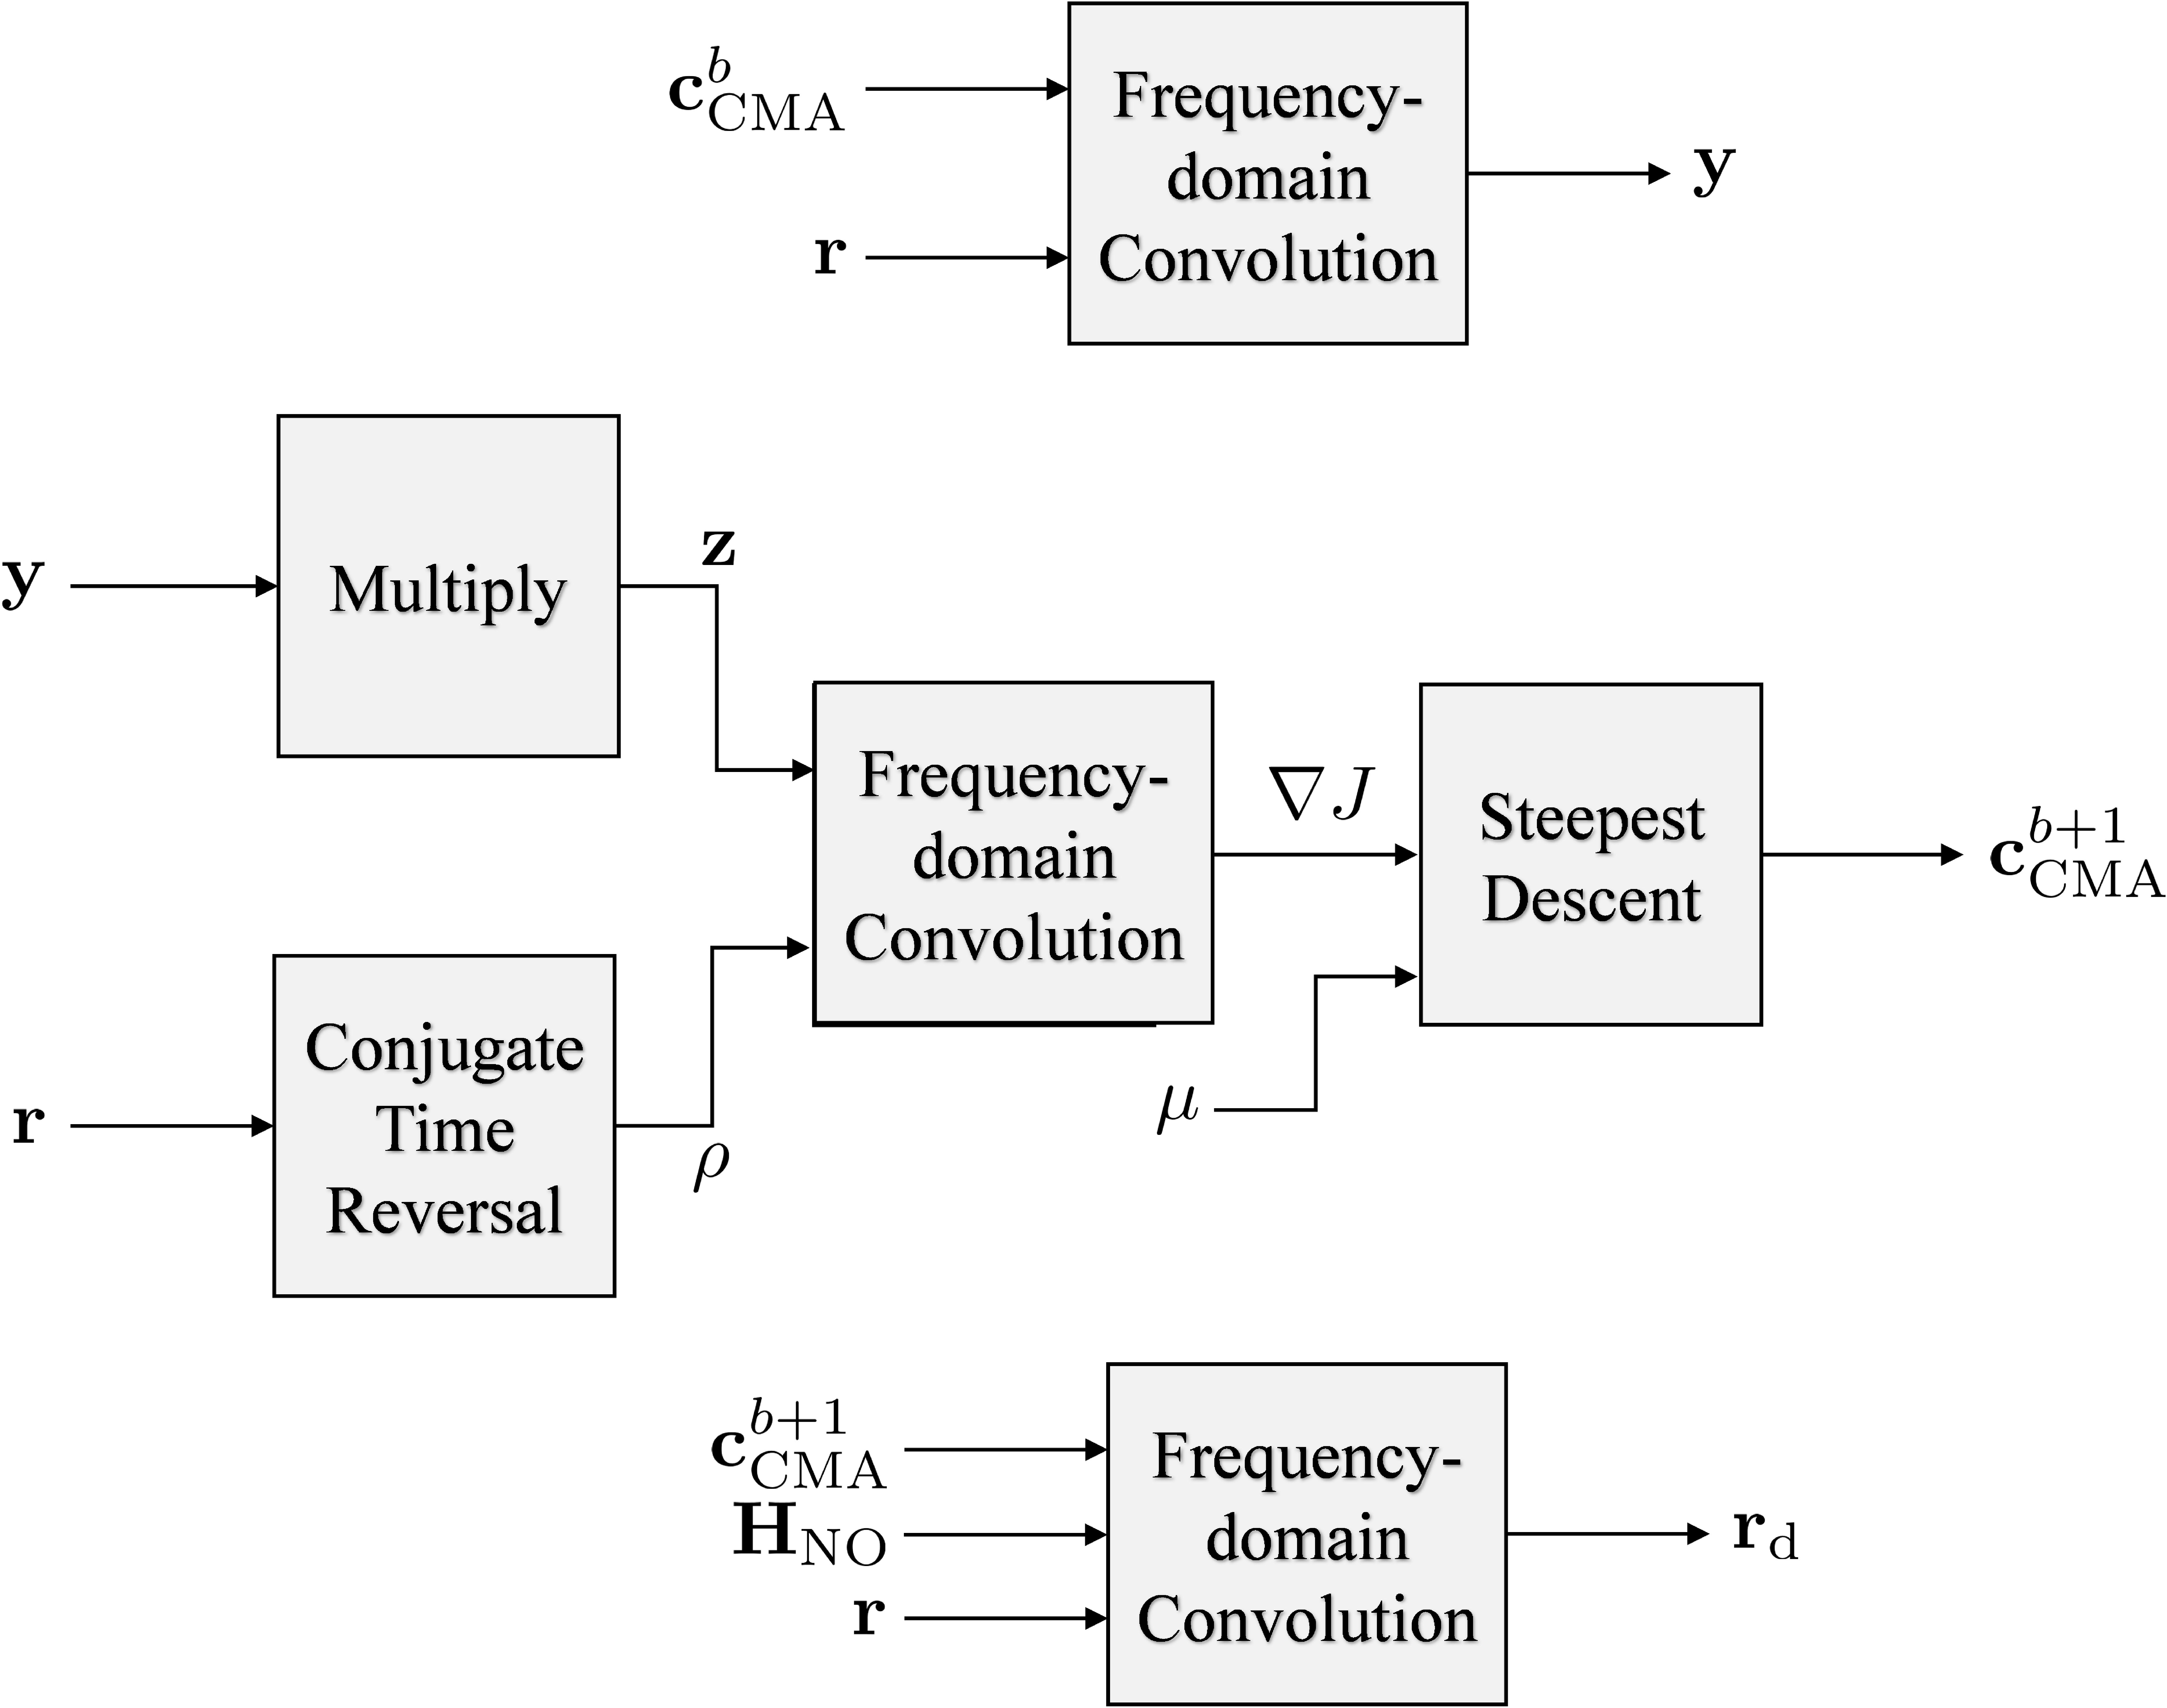
\includegraphics[width=8.34in/100*55]{figures/eq_GPUimplementation/blockCMA.pdf}
	\caption{Block Diagram showing how the CMA equalizer filter is implemented in the GPU using frequency-domain convolution twice per iteration.}
	\label{fig:blockCMA}
\end{figure}
\begin{table}
\caption{Two different algorithms were explored to compute the cost function gradient $\nabla J$.}
\begin{center}
\begin{tabular}{lll}
	\toprule
	CMA	Iteration Algorithm		& Execution Time (ms)	\\ \midrule
	$\nabla J$ directly 		& 421.317				\\
	$\nabla J$ using convolution & 88.774				\\
	\bottomrule
\end{tabular}
\end{center}
\label{tab:CMAtimingComparison}
\end{table}

\section{Frequency Domain Equalizer One and Two GPU Implementation}
The Frequency Domain Equalizers (FDEs) were by far the fastest and easiest to implement in GPUs.
The FDE1 and FDE2 block diagrams look just like the frequency-domain convolution block diagram in Figure \ref{fig:Conv3} except that complex multiplication is now complex multiplication and division.
\subsection{Frequency Domain Equalizer One}
FDE1 is the frequency-domain equivalent to the MMSE equalizer from Equation \eqref{eq:FDE1}
\begin{equation}
C_\text{FDE1}(e^{j\omega_k}) = \frac{\hat{H}^\ast(e^{j\omega_k})}  {|\hat{H}(e^{j\omega_k})|^2  +  \frac{1}{\hat{\sigma}^2_w}} \quad
\omega_k = \frac{2\pi}{N_\text{FFT}} \;
\text{for} \;
k=0,1,\cdots,N_\text{FFT}-1
\label{eq:FDE1_imp}
\end{equation}
where $N_\text{FFT} = 16$,$384$ points. Since FDE1 is applied in the frequency domain, the FFT of the received signal $R(e^{j\omega_k})$ is computed and the signal is equalized by performing a $N_\text{FFT}$ point-to-point complex multiplication and division.
The pre-computed FFT of the detection filter $\hat{H}^\ast(e^{j\omega_k})$ is also applied in the point-to-point complex multiplication and division.
The FFT of the equalized and detected signal is
\begin{equation}
R_\text{d1}(e^{j\omega_k}) = \frac{R(e^{j\omega_k}) \hat{H}^\ast(e^{j\omega_k}) H_{\text{NO}}(e^{j\omega_k})}  {|\hat{H}(e^{j\omega_k})|^2  +  \frac{1}{\hat{\sigma}^2_w}} \quad
\omega_k = \frac{2\pi}{N_\text{FFT}} \;
\text{for} \;
k=0,1,\cdots,N_\text{FFT}-1.
\label{eq:FDE1_applied}
\end{equation}



\subsection{Frequency Domain Equalizer Two}
FDE2 is the frequency-domain equivalent to the MMSE equalizer from Equation \eqref{eq:FDE2}
\begin{equation}
C_\text{FDE2}(e^{j\omega_k}) = \frac{\hat{H}^\ast(e^{j\omega_k})}  {|\hat{H}(e^{j\omega_k})|^2  +  \frac{\Psi(e^{j\omega_k})}{\hat{\sigma}^2_w}} \quad
\omega_k = \frac{2\pi}{N_\text{FFT}} \;
\text{for} \;
k=0,1,\cdots,N_\text{FFT}-1
\label{eq:FDE2_imp}
\end{equation}
where $N_\text{FFT} = 16$,$384$ points. Since FDE2 is applied in the frequency domain, the FFT of the received signal $R(e^{j\omega_k})$ is computed and the signal is equalized by performing a $N_\text{FFT}$ point-to-point complex multiplication and division.
The pre-computed FFT of the detection filter $\hat{H}^\ast(e^{j\omega_k})$ is also applied in the point-to-point complex multiplication and division.
The FFT of the equalized and detected signal is
\begin{equation}
R_\text{d1}(e^{j\omega_k}) = \frac{R(e^{j\omega_k}) \hat{H}^\ast(e^{j\omega_k}) H_{\text{NO}}(e^{j\omega_k})}  {|\hat{H}(e^{j\omega_k})|^2  +  \frac{\Psi(e^{j\omega_k})}{\hat{\sigma}^2_w}} \quad
\omega_k = \frac{2\pi}{N_\text{FFT}} \;
\text{for} \;
k=0,1,\cdots,N_\text{FFT}-1.
\label{eq:FDE2_applied}
\end{equation}

Figures \ref{fig:blockFDE1} and \ref{fig:blockFDE2} show the block diagrams for GPU implementation of FDE1 and FDE2.
As expected, these figures look just like the frequency-domain convolution block diagrams shown in Figure \ref{fig:Conv3}.
Table \ref{tab:FDEtimingComparison} shows the execution times for calculating and applying FDE1 and FDE2.
\begin{table}
\caption{Execution times for calculating and applying Frequency Domain Equalizer One and Two.}
\begin{center}
\begin{tabular}{lll}
	\toprule
	Algorithm						& Execution Time (ms)	\\ \midrule
	Frequency Domain Equalizer One 	& 57.156				\\
	Frequency Domain Equalizer Two	& 58.841				\\
	\bottomrule
\end{tabular}
\end{center}
\label{tab:FDEtimingComparison}
\end{table}
\begin{figure}
	\centering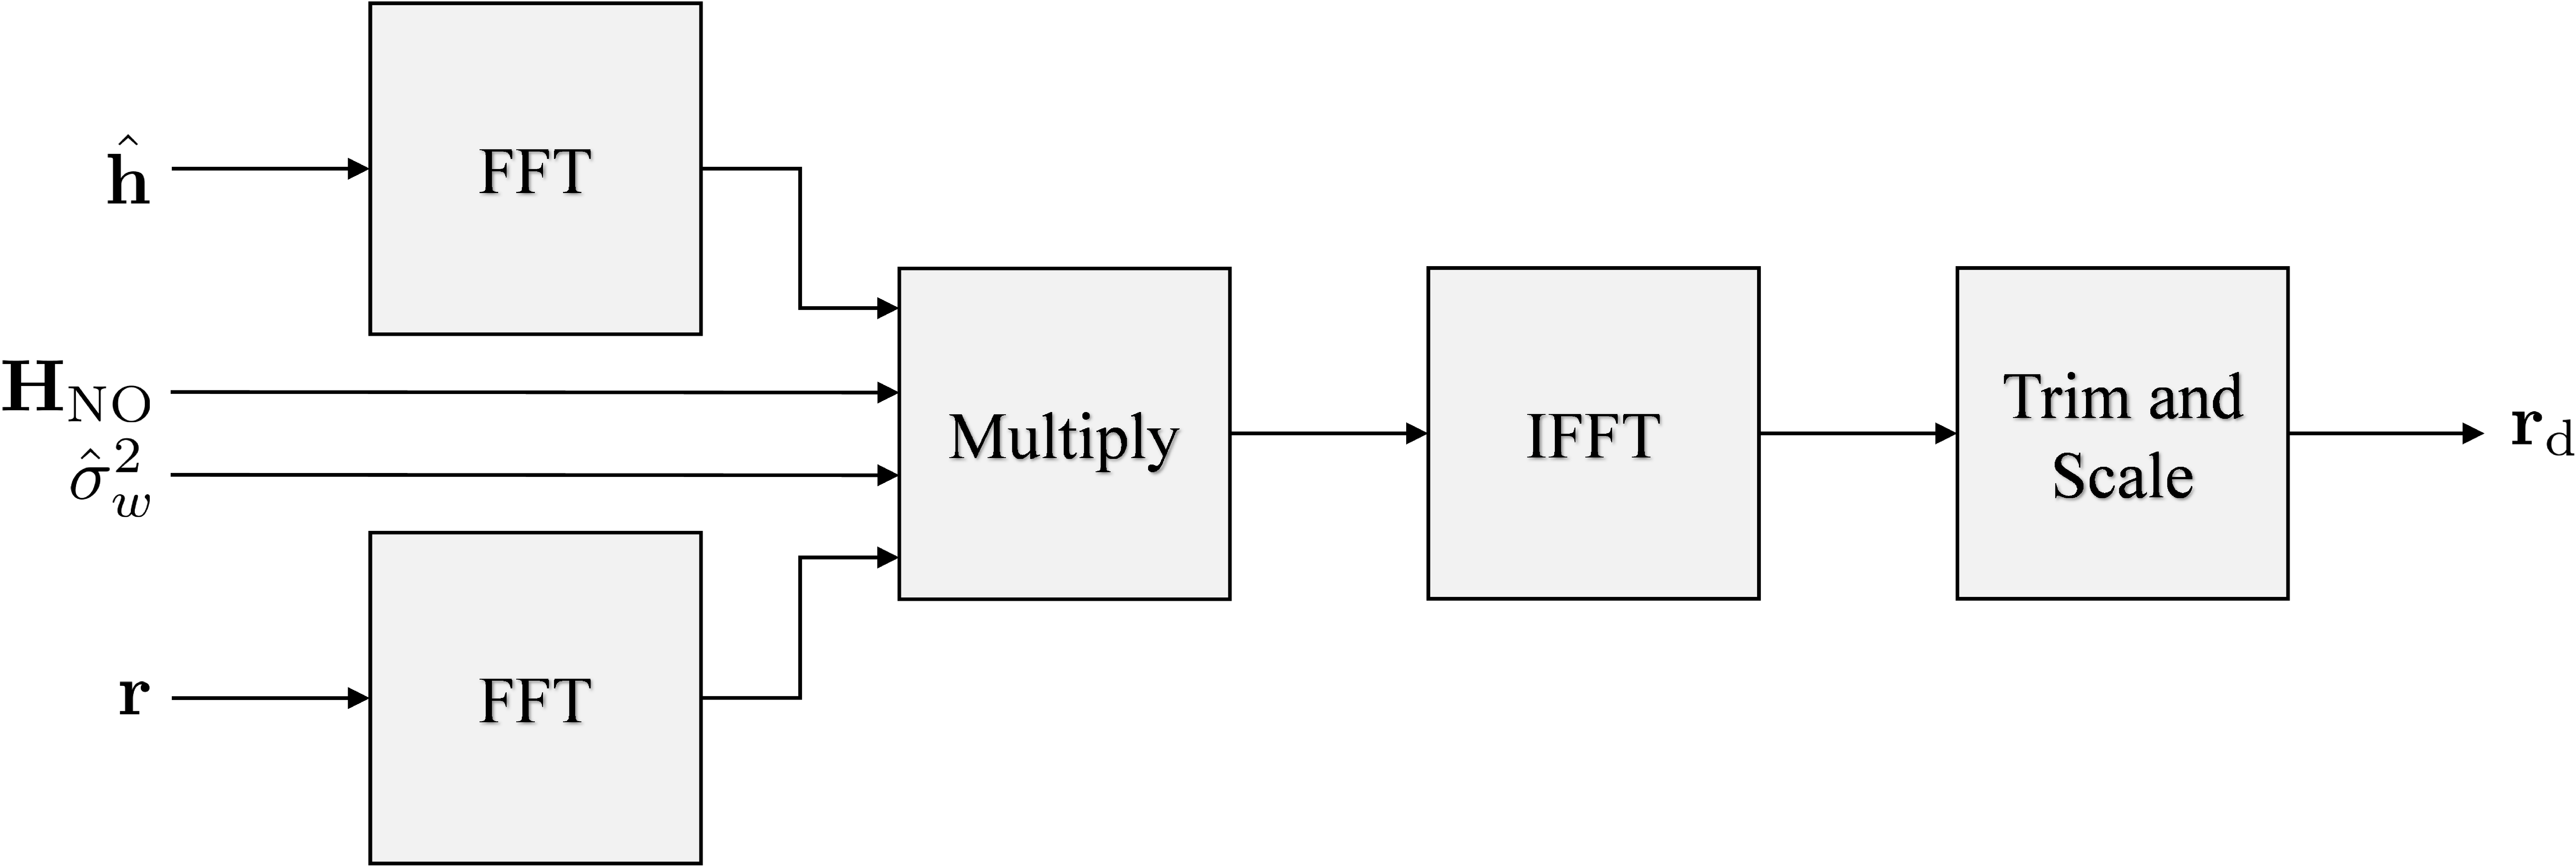
\includegraphics[width=9.73in/100*55]{figures/eq_GPUimplementation/blockFDE1.pdf}
	\caption{Block diagram showing Frequency Domain Equalizer One is implemented in the frequency domain in GPUs.}
	\label{fig:blockFDE1}
\end{figure}
\begin{figure}
	\centering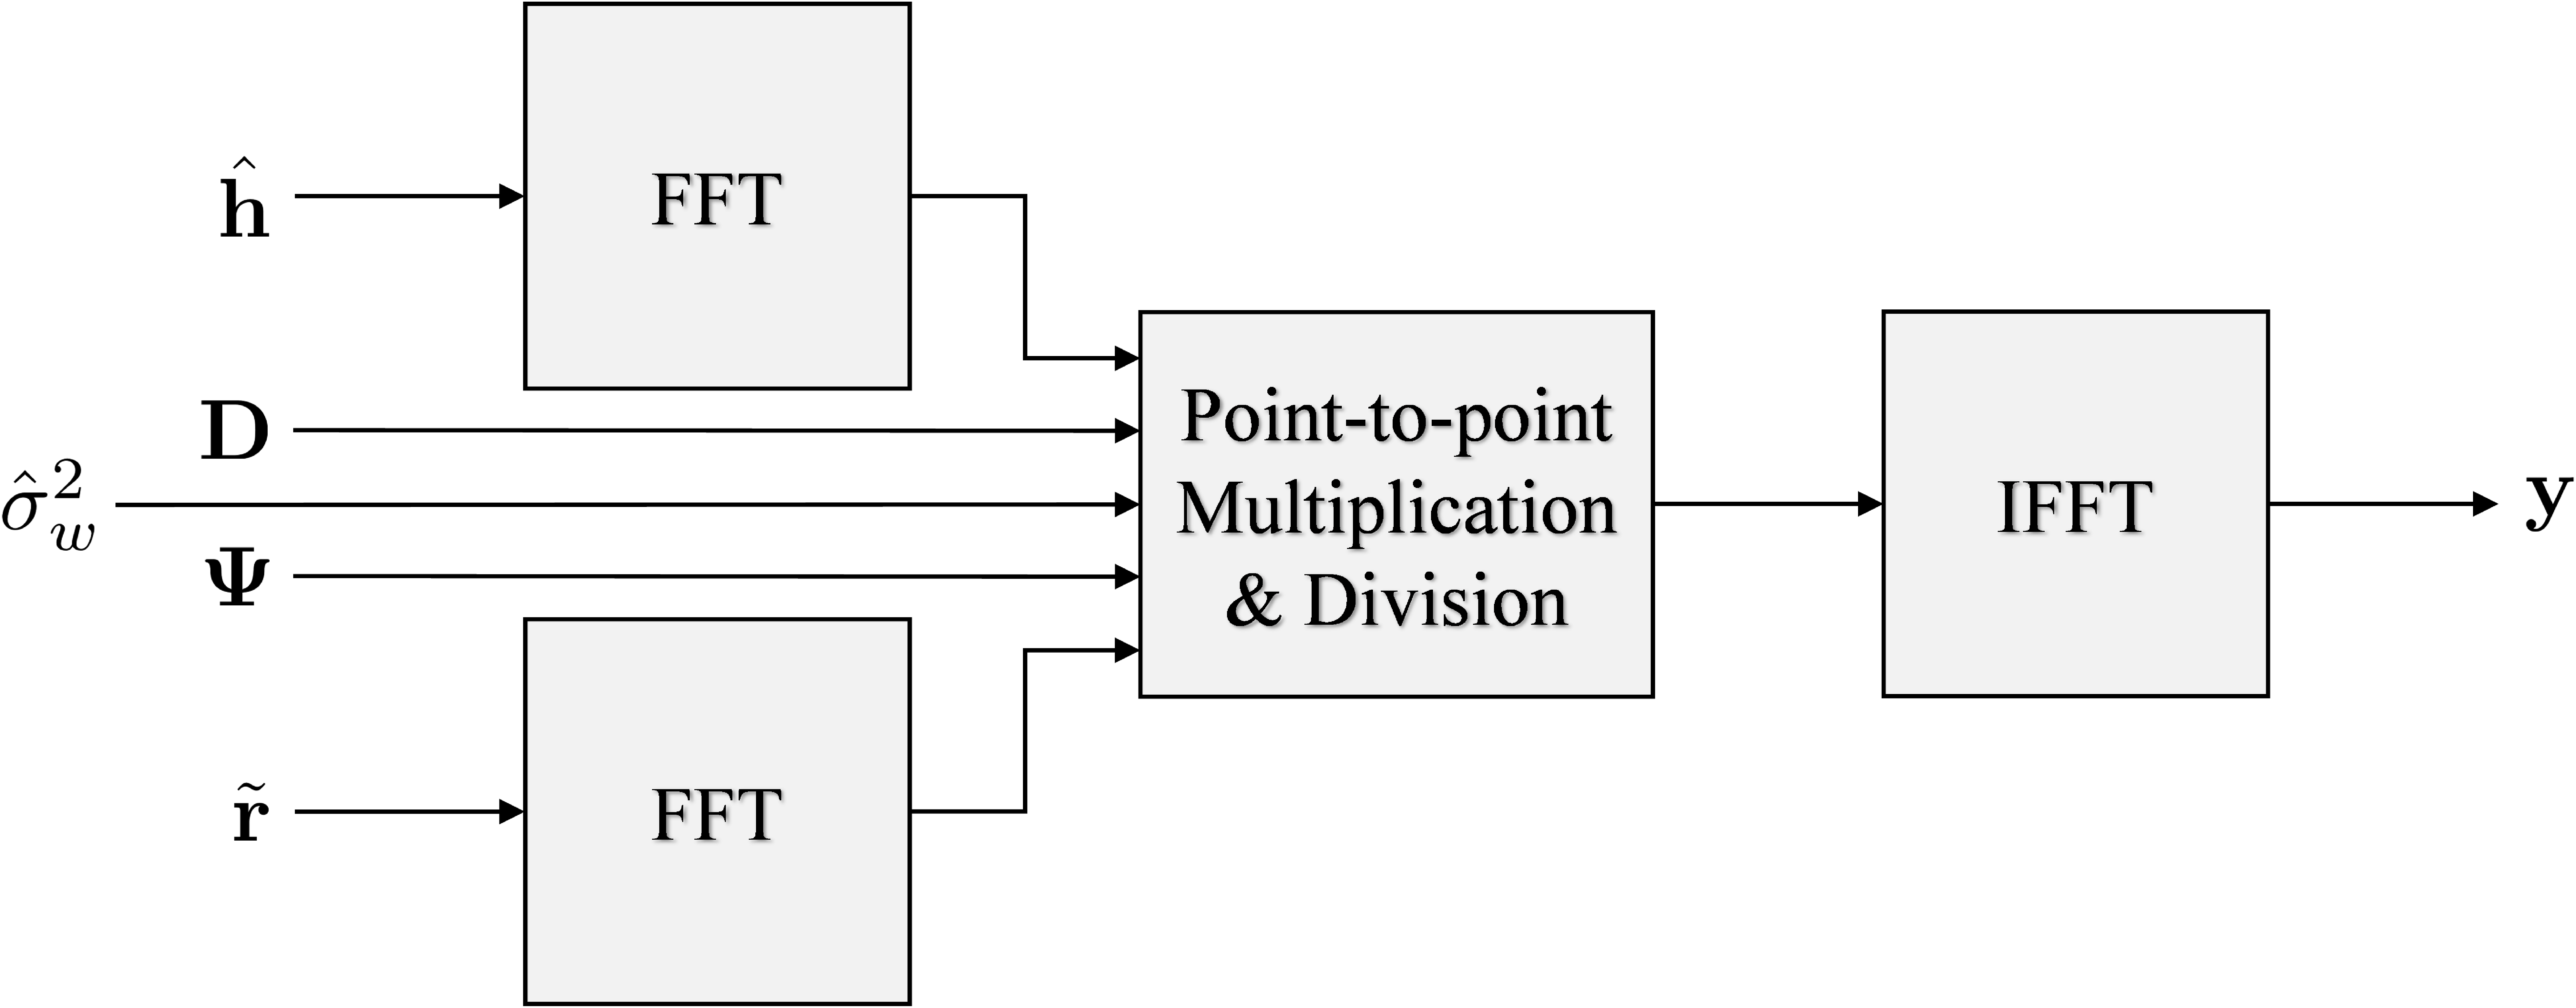
\includegraphics[width=10.03in/100*55]{figures/eq_GPUimplementation/blockFDE2.pdf}
	\caption{Block diagram showing Frequency Domain Equalizer Two is implemented in the frequency domain in GPUs.}
	\label{fig:blockFDE2}
\end{figure}





